\documentclass[12pt, a4paper]{article}

\usepackage{setspace, graphicx, caption, color, float}
\usepackage{amsmath}
\usepackage{amsfonts}
\usepackage{amssymb}
\usepackage{amsthm}
\usepackage{amstext} %to enter text in mathematical formulae
\usepackage{algorithm}%puts the psuedo code in a float box
\usepackage[retainorgcmds]{IEEEtrantools}
\usepackage{natbib}
\usepackage{rotating} %rotating text
\usepackage{multirow} %connecting columns in tables
\usepackage{multicol}
\usepackage{longtable}
\usepackage{makecell}
\usepackage{hyperref} % for linking refferences to supps
\usepackage{lineno} % for line numbers, need it after amsmath

%page set up
\usepackage[left=2.5cm,top=2.5cm,right=2.5cm, bottom=2.5cm,nohead]{geometry}
\doublespacing
%paragraph formatting
\setlength{\parskip}{12pt}
\setlength{\parindent}{0cm}

\linenumbers

\begin{document}
Title: Optimal control in the face of evolving resistance by hiding portions of the population from selection.

Shaun R. Coutts, Helen Hicks, Alexa Varah, Kwadjo Ahodo, Rob Frekleton, Dylan Z. Childs 

\section*{Introduction}
Controlling populations in the face evolving resistance to xenobiotics (i.e. antibiotics, herbicides, pesticides, fungicides) is one of the biggest challenges facing public health \citep{Laxm2016, Willy2017}, and food security \citep{Denh1992, Palu2001, Hick2018}. Evolved resistance also costs billions of dollars globally \citep{Livi2016, Ches2018, Hick2018}. While there have been some successes in combating resistance in public health \citep{REX2013}, resistance is still a major problem in health care \citep{Willy2017} and there has been little success in other contexts, such as food production.

Current strategies to manage resistance focus on delaying the initial evolution of resistance by reducing the population (reducing the potential for \textit{de nova} resistance mutations), and killing any resistant mutants by using a second compound \citep{Denh1992, REX2013}. Multiple compounds are either stacked (used at the same time) or cycled in sequence. While these strategies can be effective in delaying the initial evolution of resistance they may be counter-productive if xenobiotic resistance is already present, which is true of important pests of food production systems \citep{Denh1992, Hick2018} and threats to human health \citep{Willy2017}. Strategies like stacking and cycling involve the continuous (and even increased) use of xenobiotics, which can help drive existing resistance through an entire population \citep{Denh1992, Hick2018}.

In agricultural systems an alternative once resistance has evolved is integrated pest management (IPM), where chemical control is used in combination with non-chemical control such as crop rotation, cultivation and spot control (which can involve broad spectrum xenobiotics or mechanical control). While the concept of integrated pest management is well established \citep{Bott1979}, finding good IPM strategies is challenging \citep{Dana2014, Chal2015}. Management tools need to be used in the correct combination and sequence to be most effective. This results in a very large number of potential IPM strategies (i.e. different combinations and sequences), even when considering only a handful of management tools and short time horizons \citep{Chal2015}. As a result there have been few attempts to rigorously search for good IPM strategies (see \citealt{Chal2015} for an exception). More commonly optimal strategies have looked for the best allocation between a few management options \citep{EpanN2010, Meis2016, Okum2016, Buyu2017}, and none have been developed where resistance could evolve to one of the primary management tools. These are important omissions for food production systems where resistance to xenobiotics has evolved numerous times \citep{Denh1992, Palu2001} and multiple non-chemical control options are available that can used in combination to deliver cost effective control \citep{Chal2015}.      

Little is known about how robust good IPM strategies are to changes in factors such as crop yield and pest population dynamics \citep{EpanN2010}. However, previous work on the optimal control of invasive populations has found general factors that shape optimal decisions. Biologically, a population's ability to escape density dependence shifts optimal control to younger age classes \citep{Pich2012}. The degree to which eradicated regions can be re-invaded also influences the optimal control strategies \citep{Janu2011, EpaN2012}, but the exact strategy depends on the way suitable habitats are connected \citep{Chads2011}. Economic factors tend to be at least as important as biological ones in shaping the optimal control strategy \citep{EpanN2010}. In particular the relationship between the density of an invasive species and the damage it does has been found to be crucial \citep{Yoko2009}. The way that future returns are valued also strongly influences the optimal control strategy, when more value is placed on future versus present returns more intensive control is favoured \citep{EpanN2010}.

We apply a genetic algorithm to a model of resistance to two herbicides in an important weed of wheat in Europe (\textit{Alopecurus myosuroides}). [ALEXA: sentence or two here + REF on just how damaging BG is]. To allow IPM strategies we also include crop rotation, cultivation and spot control as management options. We find that good IPM strategies are highly context dependent, with crop yields, the yield penalty imposed by the weed, and parameters which control how large the population can grow, having the most influence on what makes a good IPM strategy.   

\section*{Methods}
We frame IPM as a combinatorial optimisation problem where the goal is to find a good combination of management tools, used in sequence. We use a genetic algorithm to solve this combinatorial problem \citep{Tayl2004GA, Carr2010}. Genetic algorithms cannot be checked to have found the globally optimal solution, as this would require already knowing the solution. However, genetic algorithms are efficient at weeding out comparatively poor solutions, so that over successive iterations the regions of the solution space being explored gets progressively better, resulting in a set of good (often near optimal) solutions.

Our goal is to find good IPM strategies in the face of rapidly evolving resistance, and how those strategies change in response to biological and management parameters. This problem has fours parts: i) A reward function that measures how good a given IPM strategy is based on how much that strategy cost and its effectiveness, we use net present economic value. ii) A population model that translates a given IPM strategy into a population, and thus a reward. iii) An algorithm that finds IPM strategies with higher rewards, the genetic algorithm. iv) Finally we need to relate changes in the best IPM strategy found to changes in initial conditions and model parameters. We use a meta-modelling global sensitivity analysis \citep{Cout2014} based on multi-variate boosted regression trees \citep{Mill2016}. 

\subsection*{Population model}
The population model links management actions to the response of the \textit{A. myosuroides} population, and thus wheat yields. The action $a_j$ is how the manager effects the population model, and thus the reward they get. Each action is a tuple of four sub-actions $a_j = \langle a_h, a_b, a_k, a_s \rangle$, see \nameref{app:A_space} for a description of the sub-actions and all eligible combinations of these sub-actions (i.e. the full actions space, $\mathbf{A}$). 

The processes included in the population model limit the scope of the IPM strategies found. We use a deterministic model, and so our IPM strategies can only deal with average expected population responses, ignoring demographic uncertainty, and environmental and market variability. Also, we only model herbicide resistance that is already present in the population because \textit{de nova} mutation is a fundamentally stochastic process. 

A commonly recommended \citep{REX2013} and applied \citep{Hick2018} strategy to combat resistance is to apply xenobiotics that impair different cellar pathways (i.e. modes of action), either sequentially (cycling) or concurrently (stacking). To allow this behaviour we use a discrete time, spatially implicit model, where two independent alleles ($R$ and $Q$), each confer target site resistance to a separate herbicide. The model must also be flexible enough to accommodate non-chemical control. We include a two level seed bank (to allow plowing to take seeds out of the germinating population) and model survival as a function of resistance, herbicide choice, crop choice and spot control (where the cost increases with \textit{A. myosuroides} density).

We model the \textit{A. myosuroides} population using a yearly time step, starting at the beginning of the growing season before any seeds have emerged. See Figure \ref{fig:life_cyc} for the timing of management interventions and \nameref{app:pop_model} for a full description of the model and how each sub-action affects the population. 

\begin{figure}[!ht]
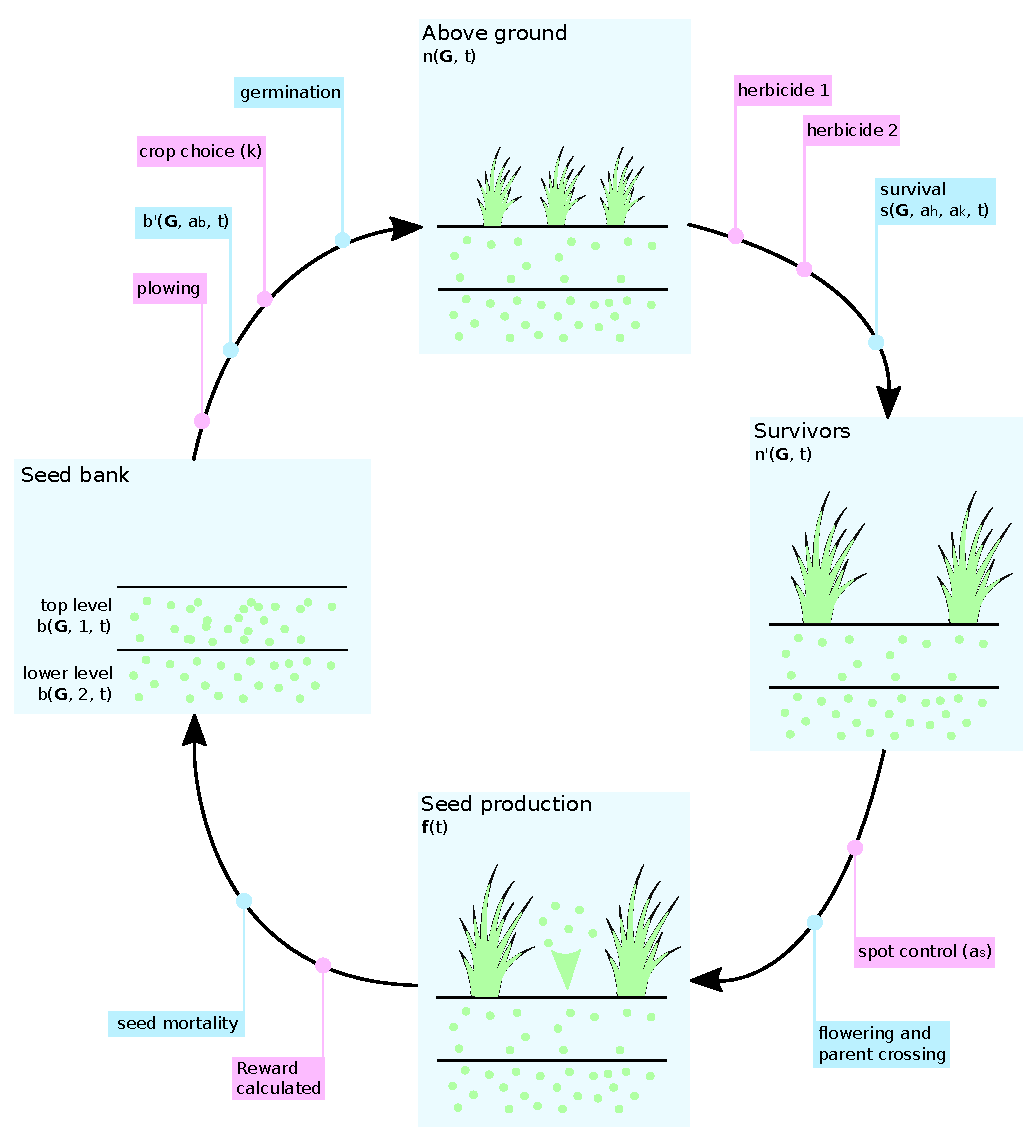
\includegraphics[scale=0.5]{MS_figs/pop_mod_2sb_scheme.pdf}
\caption{Life cycle with management interventions over the year. Pink processes are management interventions and blue processes are biological population processes.}
\label{fig:life_cyc}
\end{figure} 

\subsection*{Reward function}
The reward function measures how good an IPM strategy is, given a initial starting condition and parameter set that the model is run under. The reward function encodes the goals of a manager. We assume farmers are primarily driven by economic returns. The economic return consists of two parts, the income made from the crop and the costs of producing that crop. We assume that usual farm costs, such as buildings and machinery as constant from year to year, so we focus on gross margin, i.e. income - variable costs \citep[pp.~3--4]{Nix2016}. 

To explicitly link the above ground population to the reward function we define $N''(\mathbf{a}, n_0, t)$, the total above ground population after all control actions, at time $t$ given an initial population $n_0$ and a sequence of actions 
\begin{linenomath*}
\begin{equation}
	\mathbf{a} = \{a_j^0, a_j^1, \cdots, a_j^T\}
\end{equation}	  
\end{linenomath*} 
where $a_j^t$ is the action $a_j \in \mathbf{A}$ taken at time $t$ and $T$ is the time horizon over which management is run. We assume all returns after $T$ are ignored. The reward function is  
\begin{linenomath*}
\begin{equation}
	R(\mathbf{a}, n_0) = \sum_{t=0}^T \gamma^t \Big( Y(N''(\mathbf{a}, n_0, t)) - C(a_j^t) \Big)
\end{equation}
\end{linenomath*}
where $R(\mathbf{a}, n_0)$ is the time discounted reward for action sequence $\mathbf{a}$ given starting population $n_0$, $\gamma \in [0, 1]$ is the discount rate. When $\gamma = 0$ only the reward in the first time step is considered, when $\gamma = 1$ returns in all future time steps up to $T$ are valued equally. $Y(N''(\mathbf{a}, n_0, t))$ is the income (in \pounds /ha) from the crop chosen at time $t$ given start stating $n_0$ and following action sequence $\mathbf{a}$. $C(a_j)$ is the cost of taking action $a_j$, and is composed of the cost of controlling \textit{A. myosuroides} and other costs that depend in the crop being grown ($a_k$).   

See \nameref{app:Re_fun} for the yield and cost models for each sub-action and parameter estimation.

\subsection*{Finding good IPM strategies} 
Our goal is to find good strategists to manage black grass in the face of evolving resistance, however it is not feasible to test every combination of management options over more than a handful of years. Genetic algorithms have been used to find good solutions to this class of problem \citep{Tayl2004GA, Carr2010}. The genetic algorithm starts with an randomly generated set of action sequences, these action sequences are then iteratively improved to find a set of action sequences with a high gross margin. Genetic algorithms rely on the fact that even though the number of possible action sequences is large, many perform very poorly. The genetic algorithm explores better performing regions of the solution space more intensely. While genetic algorithms are not guaranteed to find the optimal action sequence they will find a set of actions sequences that perform well, often close to the optimal solution.   

To find good action sequences we use a genetic algorithm with knock out tournament selection, where each action sequence in a set of 1000 actions sequences is randomly paired with another, and the action sequence with the highest $R(\mathbf{a}, n_0)$ survives to help generate new action sequences. We used pair mating between survivors and N-point cross-over to produce new action sequences. After new action sequences are created there is a process of random mutation where each $a_j^t$ is changed to another $a_j^t \in \mathbf{A}$ with probability $m = 0.03$. The algorithm used is given in \nameref{app:GA}.        

\subsection*{Finding which initial conditions and model parameters lead to which IPM strategies}
It is unlikely a given IPM strategy will perform well in all scenarios. To find the parameters and initial conditions ($n_0$) that shaped the IPM strategy with the highest reward, we extend the meta-modelling approach to global sensitivity analysis outlined in \citet{Cout2014}, to multivariate time series outputs (i.e. the sequences of the four sub actions). We: i) ran the genetic algorithm under 15000 different parameter sets and initial conditions, generated with Latin hyper-cube sampling (see Table \ref{tab:pars} for upper and lower limits of each parameter), ii) used Longest Common Sub-Sequence \citep{Tooh2015} as a measure of distance between these action sequences, iii) projected the resulting distance matrix into an 8D solution space using non-metric multi-dimensional scaling (implemented in the 'ecodist' R package; \citealt{Gosl2007}), iv) predicted where each IPM solution sat in the solution space using multi-variate boosted regression tree \citep{Mill2016}, where the model parameters and initial conditions were predictors. See \nameref{app:meta_mod} for details.

It was this multi-variate boosted regression tree we interrogated to find which parameters and initial conditions were important for changing the best IPM strategy found--using relative influence and partial dependence plots \citep{Mill2016}.    

% table of parameters and ranges used
\begin{longtable}{c c c p{5cm} p{4cm}}
	\caption{Parameter descriptions and the range each parameter was tested over}
	\label{tab:pars}
	\\
	\hline
	\makecell{\textbf{Para-}\\\textbf{meter}} & \textbf{Units} & \textbf{Range} & \textbf{Description} & \textbf{Source} \\
	\hline
	\endhead
	\multicolumn{5}{l}{\textit{Population Model  see \nameref{app:pop_model}}}\\
	$\phi_e$ & prob. & 0.45--0.6 & germination probability & \citet{Colb2006} \\ 
	$\phi_b$ & prob. & 0.2--0.86 & Probability a seed survives one year & \citet{Colb2006}, \citet{Thom1997}, \citet{Cava1999}\\
	$s_0$ & prob. & fixed 0.99 & Survival probability without herbicide & Assumed fixed and high so density effects only expressed through fecundity.\\
	$\theta$ & prob. & 0.7--1 & \multicolumn{2}{l}{\parbox[t]{9cm}{Proportion of \textit{A. myosuroides} population exposed to herbicide under sub-action $a_h$ = herb R, herb Q or both. plants may be missed spatially or temporally, or spraying may be affected by rain. Tested over wide range.}} \\       
	$s_h$ & prob. & 0.01 & Survival of susceptible \textit{A. myosuroides} exposed to herbicide ($a_h$ & herbicide assumed to be effective.\\
	$\alpha$ & prob. & 0.22--0.04 & Survival probability under the alternative crop ($a_k$ = alt), spring barley. & \citet{Lutm2013}\\
	$\beta$ & prob. & 0.05--0.2 & Survival under spot control (sub-action $a_s$), for example because plants are missed & tested over wide range.\\
	$f_m$ & \makecell[t]{seeds$\cdot$\\plant$^{-1}$} & 30--300 & \multicolumn{2}{l}{\multirow{2}{9cm}{\parbox[t]{9cm}{Number of seeds produced when density is 0 ($f_m$) and The effect of density on seed production ($f_d$) interact to determine maximum population size. Values chosen to keep the max population close to the maximum population seen in \citet{Quee2011} so yield is not extrapolated outside the observed range.}}} \\
	$f_d$ & $\frac{1}{plants\cdot ha^{-1}}$ & 0.001--0.0001 &  \\\\\\\\\\\\
	$I$ & prob. & 0.5--0.9 & The proportion of seed moved between seed bank levels by ploughing (sub-action $a_b$) & \citet{Grun1999} \\ 
	\multicolumn{5}{l}{\textit{Reward function see \nameref{app:Re_fun}}}\\
	$\gamma$ & & 0.75--1 & discount rate on future returns & tested over wide range\\
	$Y_0$ & \pounds $\cdot ha^{-1}$ & 968--1758 & Yield from winter wheat when \textit{A. myosuroides} is absent. & Upper limit upper 95\% confidence interval from fitted yield function (\nameref{app:Re_fun}). Lower limit from low production scenario \citet[pp.~9]{Nix2016}.\\
	$Y_D$ & \makecell[t]{\pounds$\cdot$plant$\cdot$\\$ha^{-1}$} & 0.0002--0.006 & reduction in yield cuased by each \textit{A. myosuroides}. & 95\% confidence interval from fitted yield function, see \nameref{app:Re_fun}. \\
	$\vartheta$ & \pounds$\cdot ha^{-1}$ & 672--920 & Yield of spring barley, an alternative crop commonly used to control \textit{A. myosuroides}. & \citet[pp.~12]{Nix2016}\\
	 $\varpi$ & prop. & 0.85--1 & proportion of yield achieved if crop $a_k$ is repeated & \citet[pp.~9]{Nix2016} \\
	 $\eta_h$ & \pounds$\cdot ha^{-1}$ & 50--100 & Cost of a single herbicide application & \citet[pp.~9]{Nix2016}\\
	 $\eta_b$ & \pounds$\cdot ha^{-1}$ & 55--92 & Cost of ploughing & \citet[pp.~202]{Nix2016}\\
	 $\eta_s^0$ & \pounds$\cdot ha^{-1}$ & 10--100 & Cost of spot control even when \textit{A. myosuroides} density is 0 & tested over wide range\\
	 $\eta_s$ & \makecell[t]{\pounds$\cdot$plant$\cdot$\\$ha^{-1}$} & 10--100 & Increase in spot control cost for each \textit{A. myosuroides} & tested over wide range\\
	 $\eta_\text{wheat}$ & \pounds$\cdot ha^{-1}$ & 383 & Cost of growing winter wheat not associated with \textit{A. myosuroides} control & \citet[pp.~9]{Nix2016}\\ 
	 $\eta_\text{alt}$ & \pounds$\cdot ha^{-1}$ & 273 & Cost of growing the alternative crop, spring barley. & \citet[pp.~12]{Nix2016}\\	    
	 $\eta_\text{fal}$ & \pounds$\cdot ha^{-1}$ & 36 & Cost of a fallow rotation. Based on two applications of glyphosate to control any germinating \textit{A. myosuroides}. &  \citet[pp.~202 and 284]{Nix2016}\\
	\multicolumn{5}{l}{\textit{Initial Conditions}}\\
	$R_\text{int}$ & & 0--1 & Initial frequency of R alleles & \\
	$Q_\text{int}$ & & 0--1 & Initial frequency of Q alleles & \\ 
	$N_\text{int}$ & & \makecell[t]{100--\\100000} & Initial number of seeds in each level of the seed bank & \\
	\hline
\end{longtable}

\section*{Results}
IPM strategies with high gross margins were dependent on the yield of winter wheat ($Y_0$), the slope of the yield function ($Y_D$) and a set of parameters that control how large the seed bank  can become, $f_{max}$, $f_d$ and $\phi_b$ (Figure \ref{fig:rel_inf}). Discount rate ($\gamma$), initial resistance to the most effective herbicide, and the cost and effectiveness of spot control, all had moderate effects on at least two dimensions. There are some interesting exclusions from this list. Despite plowing forming a part of many good IPM strategies its cost and effectiveness have very little influence on how it is used. This suggests that if it is a good idea to plow, it is worth doing regardless of the cost and how much of the seed bank it inverts (at least within the limits we tested). \textit{A prior} we had thought that the initial population would have a large effect on the structure of a good IPM strategy, since weed control at very high population densities often looks very different to managing small populations. However our analysis suggests that initial population size had very little relative influence. If other parameters are such that effective control is possible even large seed banks can be quickly reduced, and if they are not small populations can quickly grow to large ones.   
     
\begin{figure}[!ht]
	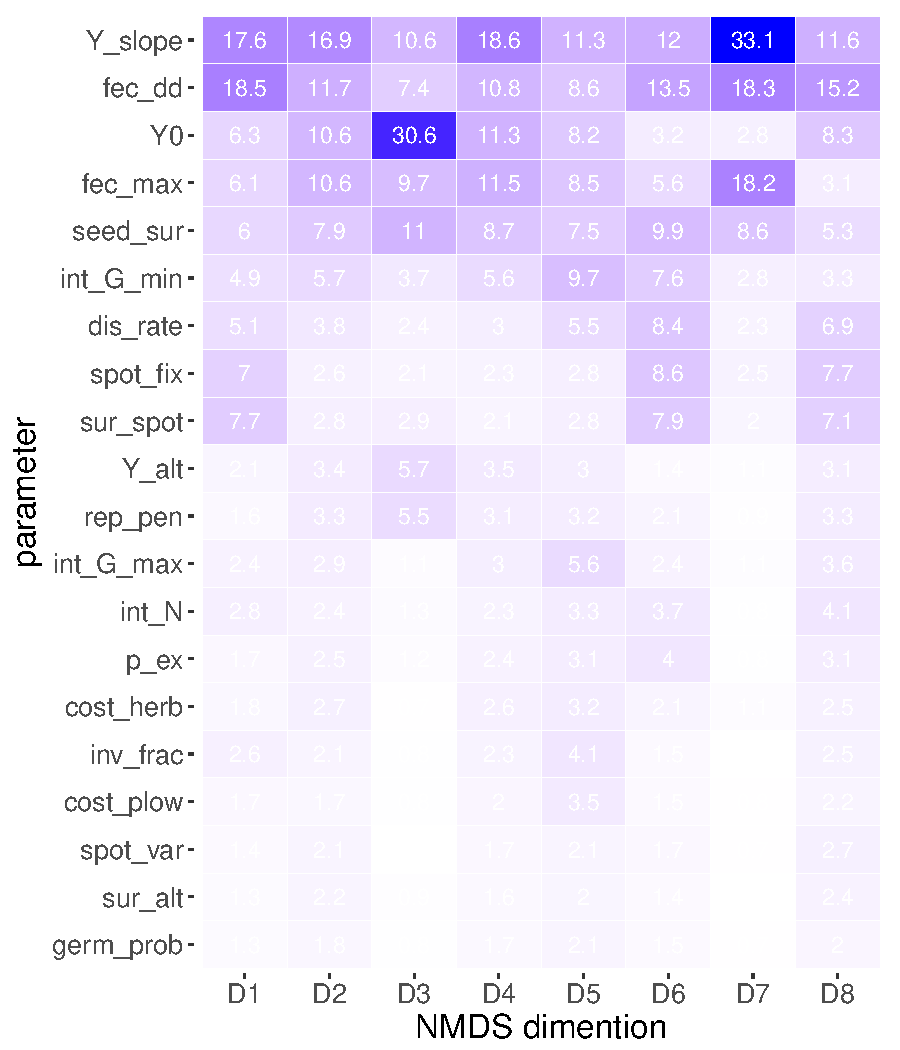
\includegraphics[width=90mm]{MS_figs/rel_inf_matrix_plot.pdf}
	\caption{Relative influence (relative reduction in squared error [mvtb REF]) of each parameter. Values are scaled 0 to 100, with higher values indicating parameters (rows) that had more influence on where solutions sat in each dimension of the solution space (columns). Parameters could have a larger effect on the structure of a good IMP strategy by either being very influential in one dimension (e.g. $Y_0$), or having moderate influence across several dimensions (e.g. $f_d$).}
	\label{fig:rel_inf} 
\end{figure}

We examine how these key parameters change the structure of IPM strategies with high gross margin. We plot the effect in combinations since interactions between parameters are important.

When the slope of the yield function ($Y_D$) was low the best IPM strategy found was to do nothing, as the yield penalty incurred by even high densities of \textit{A. myosuroides} did not incur a large enough cost to justify spending on control (although crop rotation was carried out when the yields of winter wheat were low. This was true across a wide range of values for other parameters. 

When the slope of the yield function was high, and winter wheat yield decreased sharply with increasing \textit{A. myosuroides} density, a wider range of IPM strategies were found (Figure \ref{fig:Y0_YD}). When winter wheat yields were high (Figure \ref{fig:Y0_YD}a,b) IPM strategies centred on growing winter wheat, and using intensive management to reduce the density of \textit{A. myosuroides}. When at least one effective herbicide was available this involved all non-crop options (Figure \ref{fig:Y0_YD}b). When there was no effective herbicide (due to high initial levels of resistance) plowing was the only action used to try and control the seed bank. When winter wheat yields were low (Figure \ref{fig:Y0_YD}c,d), spring crop dominated rotations and spot control were favoured, with more tactical use of herbicide when at least one effective compound was available (\ref{fig:Y0_YD}d).              
\begin{figure}[!ht]
	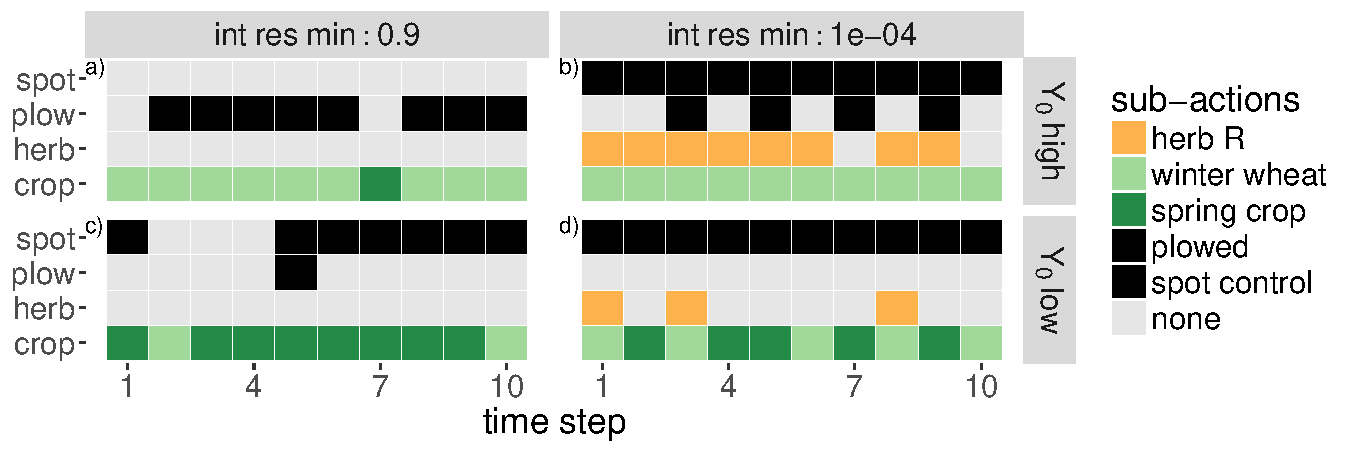
\includegraphics[width=120mm]{MS_figs/MS_act_seq_slope_Y0.pdf}
	\caption{The good IPM strategies under high (\pounds 1668$\cdot$ha$^{-1}$) and low (\pounds 986$\cdot$ha$^{-1}$) values of $Y_0$ (yield of winter wheat with no \textit{A. myosuroides}). The left column shows IPM strategy when there is high initial resistance to both herbicides and the right column shows IPM strategy when initial resistance to one herbicide is low. The effect of \textit{A. myosuroides} density on winter wheat yield ($Y_D$) is 0.0062 \pounds$\cdot$plant$^{-1}\cdot$ha$^{^-1}$. Low values of $Y_D$ lead to no control being the best IPM strategy.}
	\label{fig:Y0_YD} 
\end{figure}

Intensive management to reduce the seed bank was only used when discount rates were high (Figure \ref{fig:dis_rate}). Recall that although we only show the first 10 years of IPM strategy, the discounted returns over 25 years are considered by the genetic algorithm. With low winter wheat yields, high \textit{A. myosuroides} seed banks were managed by cycling herbicides to reduce the above ground population, and alternating winter wheat and spring crops. In order to reduce the seed bank spot control was needed post plowing and herbicide to keep the seed producing population of \textit{A. myosuroides} very low.
\begin{figure}[!ht]
	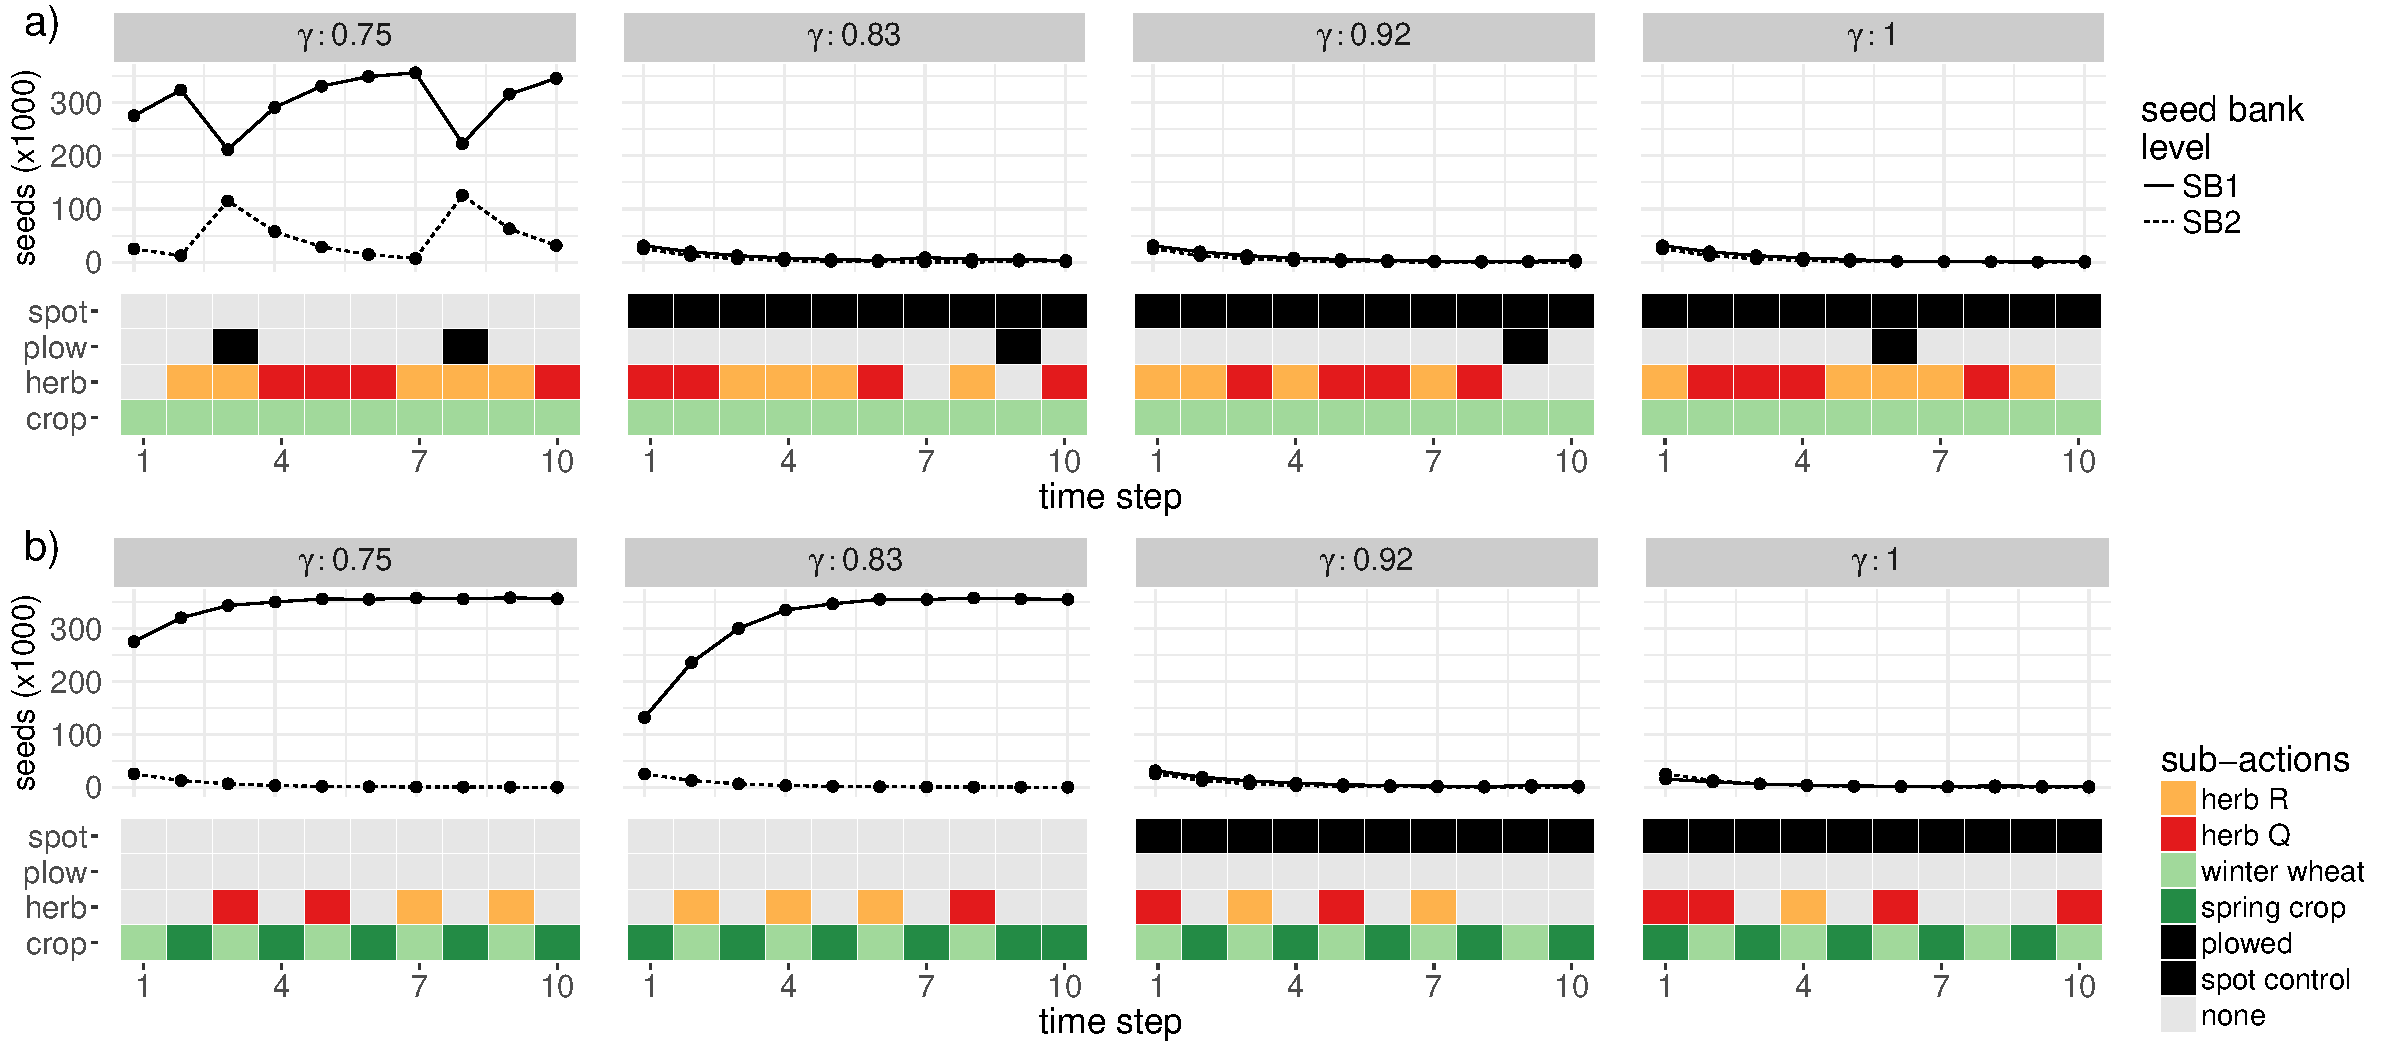
\includegraphics[height=90mm]{MS_figs/dis_rate_SB_strat.pdf}
	\caption{The effect of discount rate ($\gamma$) on the seed bank and IPM strategy (tile plots) when yields from winter wheat are high (a) and low (b). In both cases the slope of the yield function ($Y_D$) is high, with a large effect of \textit{A. myosuroides}. Initial resistance was low for both herbicides.}
	\label{fig:dis_rate} 
\end{figure}

When both herbicides were effective the preference was to cycle between them, however even this did not prolong their continued use by much. Even when both $R$ and $Q$ started at frequencies of 1 in 20,000 alleles (Figure \ref{fig:int_res}a) continued herbicide use raised those frequencies to 1 in 50 within 10 time steps. This frequency provided enough variation for selection to rapidly act on (Figure \ref{fig:int_res}c).
\begin{figure}[!ht]
	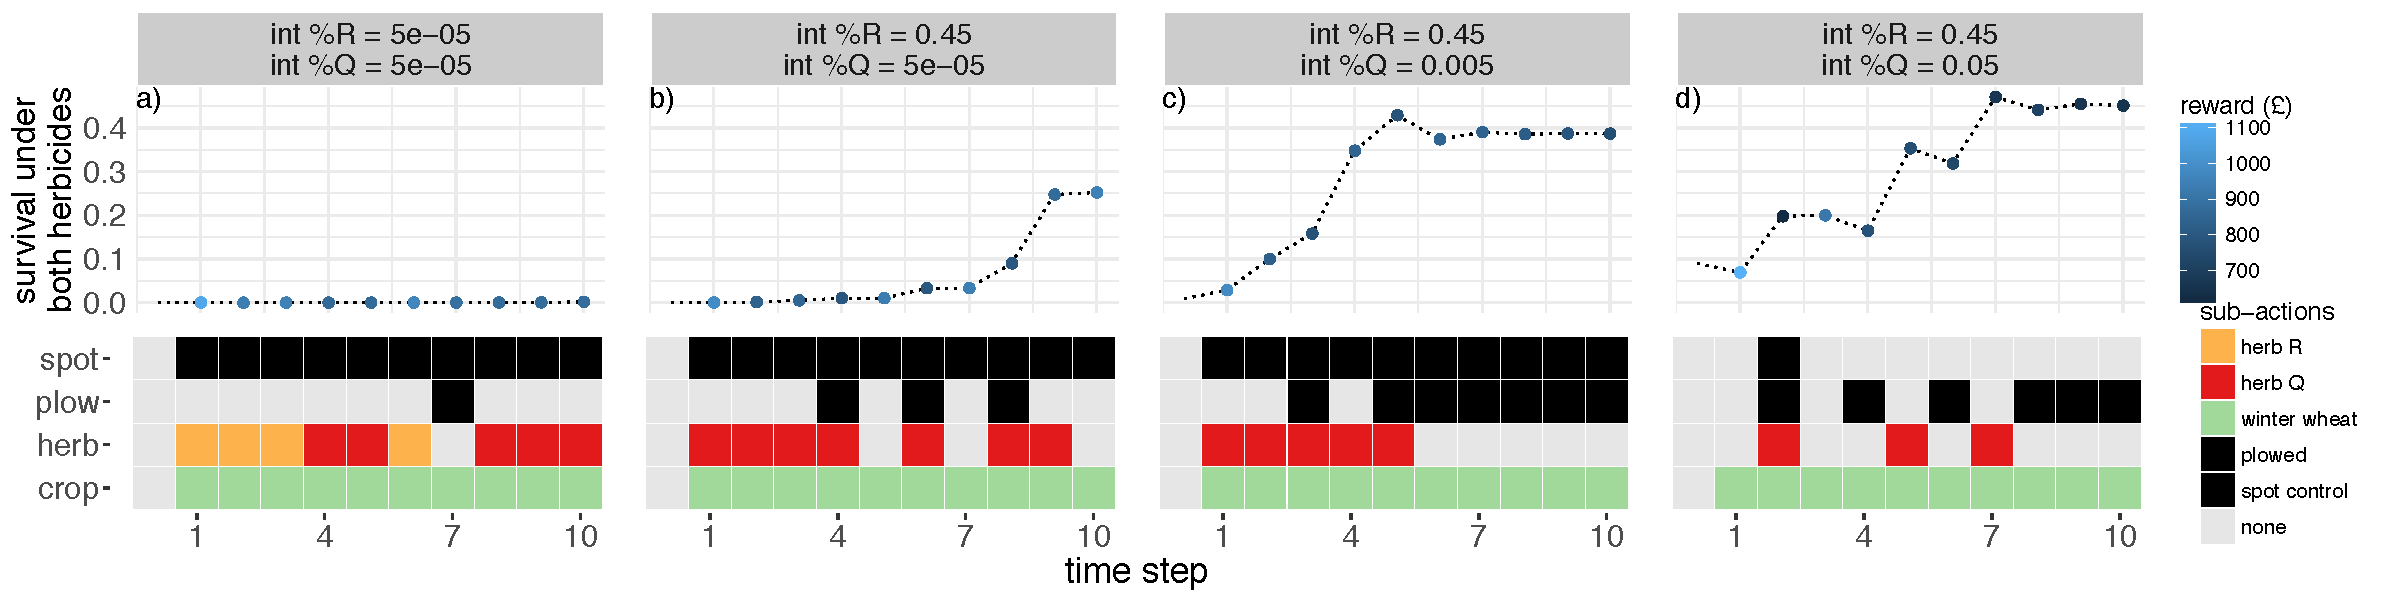
\includegraphics[width=160mm]{MS_figs/int_res_strat_resist.pdf}
	\caption{The effect of initial resistance on the selected IPM strategy (tile plots) and the evolution of herbicide resistance (\% survival to under both herbicides). Lighter coloured points indicate higher reward (gross margin) obtained in that time step. In this case $Y_0 = 1668$ (high winter wheat yield) and $Y_D = 0.0062$ (high yield penalty).}
	\label{fig:int_res} 
\end{figure}

Even when initial frequencies of resistance to the remaining effective herbicide was low (1 in 200; Figure \ref{fig:int_res}c) initial continual use quickly drove the evolution of resistance to levels where herbicide use was greatly reduced after just five generations. As the initial frequency of resistance to the remaining effective herbicide ('herb Q' in this case) increased, even moderate herbicide use drove the rapid evolution of herbicide resistance. With an initial frequency of resistance alleles of 1 in 20 even three herbicide applications were enough to increase resistance to the point where applying both herbicides would result in 40\% survival (Figure \ref{fig:int_res}d). Once this situation was reached, gross margin was reduced by a quarter compared to returns with low resistance. 

\section*{Discussion}
We found that IPM strategies were highly dependent on the yield function, relating the density of \textit{A. myosuroides} to winter wheat yields, and the density that \textit{A. myosuroides} could reach (which interacts with the yield function). To a lesser extent IPM strategies were shaped by the way future returns were valued and the initial frequency of herbicide resistance in the population. The IPM strategies with the best returns ranged from doing nothing, to high intensity management. 

Herbicide use was greatly reduced when even moderate resistance evolved, which could happen after as few as five generations exposed to herbicide. This is in contrast to current management practice in this cropping system, where multiple herbicide applications a year are the norm, despite high levels of resistance \citep{Hick2018}. [HELEN: Could you flesh this out a bit by suggesting a few reasons why the difference, and cost of using ineffective herbicides]    

The key uncertainties highlighted by this work were economic. It is not surprising that economic factors shaped IPM strategies. Factors such as crop prices, harvest efficiency and costs, directly affect the gross margin of an IPM strategy. Although yield functions have been estimated for major weeds \citep{Cous1985, Doyl1986, Swin1994}, there is evidence that yield functions vary substantially between fields \citep{Swin1994, Hick2018}, and little attention has been paid this variation and understanding its causes. This poses a considerable challenge for formulating IPM strategies, as what works well in one field may not be transferable to another.             

Supporting previous work \citep{EpanN2010} we found higher values on future returns lead to more intensive IPM strategies. In agricultural systems those who own fields can benefit from long-term investments like weed control campaigns and soil conservation, whereas those who rent fields do not \citep{Wies1996, Fras2004}. [HELEN/ALEXA: have you ever seen an estimate for how many fields are rented in the UK? I would like to write something like: In the UK X\% arable fields are rented, and our finding suggests this has important implications for the level of \textit{A. myosuroides} control managers are incentivised to provide, and thus its spread [REF] and the evolution of resistance [REF].]

We make three assumptions that impact how these results can be interpreted. Firstly, the model was deterministic, so IPM strategies could not be risk averse to variability in \textit{A. myosuroides} populations and economics factors like crop prices. 

Secondly, we assume that herbicide resistance was conferred by a target site mutations that were already present in the population (although possibly at low frequencies). This is why cycling was often favoured over stacking when two effective herbicides were available, as cycling prolonged the useful life of both herbicides since the application of each was spread out. There is growing evidence that non-target site resistance, which confers cross resistance, is widespread \citep{Hick2018}. If generalized, non-target site, resistance mechanisms are present, the total amount of herbicide exposure predicts resistance level \citep{Hick2018}, and cycling will not help.

Finally we assume that herbicide is the only action that drives the evolution of resistance. Any effective management tool will impose selection pressure, and so drive resistance to that tool. In reality, the spring cropping and spot control sub-actions make heavy use of glyphosate to control \textit{A. myosuroides}. Glyphosate resistance has evolved on many separate occasions in response to prolonged, heavy use \citep{Samm2014}. As glyphosate becomes a more important part of \textit{A. myosuroides} management \citep{Hick2018} resistance is likely. [HELEN: anything missing from this para or the previous one?]         

Our results show that farmers have an economic incentive to change their management in response to changes in \textit{A. myosuroides} populations, spatial variation in its effect on wheat yields, and changes in commodity prices. [ALEXA: would be nice to conclude with a nice summary statement on what a failure to be responsive will cost farmers, the economy as whole and the environment, are at least as much as we can say at this point. Also be a good place to flag your up coming work for any things that are still unresolved. If it is all unresolved that is an important message as well I think.] 

\section*{Supplementary material}
\paragraph*{Appendix 1}
\label{app:A_space}
Action Space
\paragraph*{Appendix 2}
\label{app:pop_model}
Population Model
\paragraph*{Appendix 3}
\label{app:Re_fun}
Reward Function
\paragraph*{Appendix 4}
\label{app:GA}
Genetic Algorithm
\paragraph*{Appendix 5}
\label{app:meta_mod}
Finding Which Initial Conditions and Model Parameters Lead to Which IPM Strategies

\bibliographystyle{/Users/shauncoutts/Dropbox/shauns_paper/referencing/bes}
\bibliography{/Users/shauncoutts/Dropbox/shauns_paper/referencing/refs} 

\end{document}
